\documentclass[12pt]{article}
\usepackage{amsmath}
\usepackage{amssymb}
\usepackage{tabularx}
\usepackage{amsmath}
\usepackage{graphicx}
\usepackage{systeme}
\usepackage{nameref}
\usepackage{caption}
\usepackage{url}
\usepackage{float}
\graphicspath{ {./diagrams/} {./screens/} {./official/} }

\usepackage{setspace}
\setstretch{1.25}

\usepackage{afterpage}

\newcommand\blankpage{%
    \null
    \thispagestyle{empty}%
    \addtocounter{page}{-1}%
    \newpage}

\usepackage{listings}
\usepackage{xcolor}

\lstdefinestyle{sharpc}{language=[Sharp]C, frame=lr, rulecolor=\color{blue!80!black}}


\begin{document}
\setlength{\parindent}{0in}

\begin{titlepage}
\begin{center}

\begin{large} 
\textsc{Politecnico di Milano}
\end{large}
\\
Scuola di Ingegneria Industriale e dell’Informazione \\
Computer Science and Engineering \\
Dipartimento di Elettronica, Informazione e Bioingegneria \\

\vspace{0.8cm}
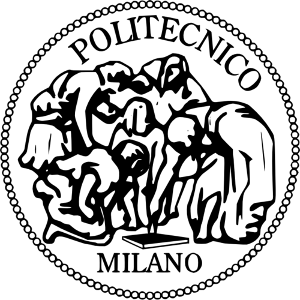
\includegraphics[width=0.4\textwidth]{poli}

\vspace{2cm}

\begin{Large}
\textbf{Fast communication training through asymmetrical multiplayer videogames}
\end{Large}

\vspace{2cm}

\begin{flushleft}
Relatore:
Prof. Marco Gribaudo
\end{flushleft}

\vspace{1cm}

\begin{flushright}
Tesi di Laurea di: \\
Jacopo Grandi, Matr. 947077
\end{flushright}

\vfill
Anno Accademico 2020/2021
\end{center}
\end{titlepage}

\clearpage

\afterpage{\blankpage}

\clearpage

\afterpage{\blankpage}

\begin{abstract}
Games can be a powerful learning tool. For instance typing games and rhythm games are genres defined by the skill they require. These games reward players for improving, pushing the players to play more and better and trying to make the experience as fun as possible. The game we developed is focused in training the communication, planning and problem solving skills of the players. The game puts the players under time pressure and requires a significant amount of information to be exchanged quickly. It also forces a half duplex communication protocol emulating a radio, such that only one player may speak at a time. The courier players will also have to solve space navigation puzzles, obstacle avoidance and local route planning; others will have to make a general plan, assign tasks and deal with multitasking. 
\end{abstract}

\clearpage

\tableofcontents

\clearpage

\section{Introduction}
Failure is an effective way to learn. This is the trial and error approach to problem solving: keep trying until a success or stop trying \cite{try}. Videogames provide an environment where the players can fail more often and reward the players who keep trying and succeed. The environment has a clear goal, such as play the correct notes \cite{rhythm} or type the correct word \cite{typing}, and a clear definition of a mistake with immediate consequences. 

\begin{figure}[H]
\begin{center}
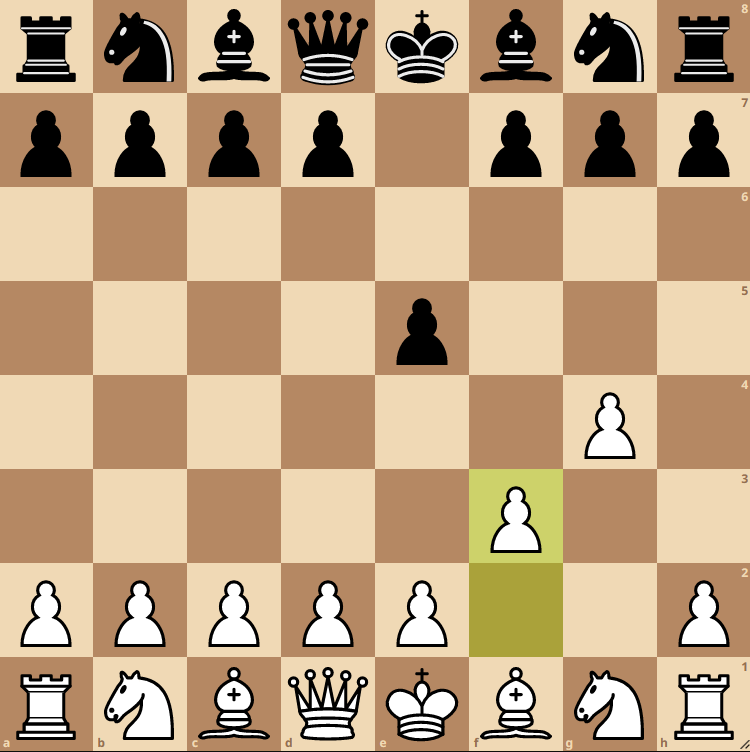
\includegraphics[height=7cm]{chess}
\end{center}
\caption{White played f3, a clear mistake as Black has Qh4 checkmate.}
\end{figure}



\paragraph{Serious games}
Videogames have been subject of study in educational research and are starting to be used by schools. For instance, Minecraft \cite{minecraft} has an educational edition with the purpose of being a platform for learning chemistry, coding and being a virtual classroom. A serious game can be defined as "Any piece of software that merges a non-entertaining purpose (serious) with a video game structure (game)" \cite{serious}. Serious games thus represent a larger set of games than educational games. Skill training games are serious games, often called exergames if they are intended to make the player do physical exercise. The game we developed is designed to be a serious game, merging the fun of playing a videogame to the tedious learning task. 

\paragraph{Skill training} 
The skills we have designed the game to train are problem-solving and communication. Videogames are a good medium to train problem-solving as stated above. Communication, chat or voice chat, is only in multiplayer games. In these games it is rarely used as a core aspect of the game and is just a platform to socialize or banter. Voice chats are often used effectively in competitive team games such as Counterstrike \cite{counterstrike} or Forged Alliance \cite{faf}, but they are not required. We required the use of a voice chat by forcing the players to exchange information that is needed to beat the game. The main difficulty of the game is to get the informations from the other players. 

\subsection{Applicable scenarios}
There are situations in which an operation team have to be guided by a remote team. This situations are common in cave exploration, cave rescues, bomb defusal, warfare and even firefighting operations in thick fog. The operation team lacks vital information to act sensibly, informations that the remote team can provide. Although, the remote team may need to ask for local data, for instance a description of the operation team surroundings, to remove uncertainties from its model of reality. If the exchange of information is slow and inefficient the operation team may have to take unnecessary risks and possibly lead to a failure, which in the situations described in the examples is catastrophic.

\subsection{Asymmetrical multiplayer}
A game has asymmetrical multiplayer when the players play the game differently. There are multiple levels of asymmetry: from a slight imbalance in the mechanics to a completely separate set of rules. In fps (first person shooter) games like Halo \cite{Halo} the players usually start with the same action set but the map can be asymmetric. Games like Starcraft \cite{starcraft} have three different races to choose from that offer wildly different strategies and gameplay, which is much more asymmetric. Keep Talking and Nobody Explodes is the most asymmetrical game in the cited games: a player defuses a virtual bomb while the other just has a printed manual on how to do it. The game we designed is an asymmetrical game because it's easier to hide information between players. They are separated in different virtual spaces, they can gather information and act differently.

\subsection{Similar games}
We analyzed more in depth a set of games that inspired the design, are good examples of serious games or feature asymmetrical multiplayer. 

\paragraph{Keep Talking and Nobody Explodes} \cite{ktne}
The game consists in defusing a ticking bomb by solving puzzles attatched to it. It's a two player game, one player is the defuser and the other has a bomb-defusal manual. The players have to exchange the puzzle state and solutions. This game fits the serious game definition. The primary purpose of the game is to entertain, but to be entertained the game requires certain skills by the players. 

\vspace{0.4cm}
\frame{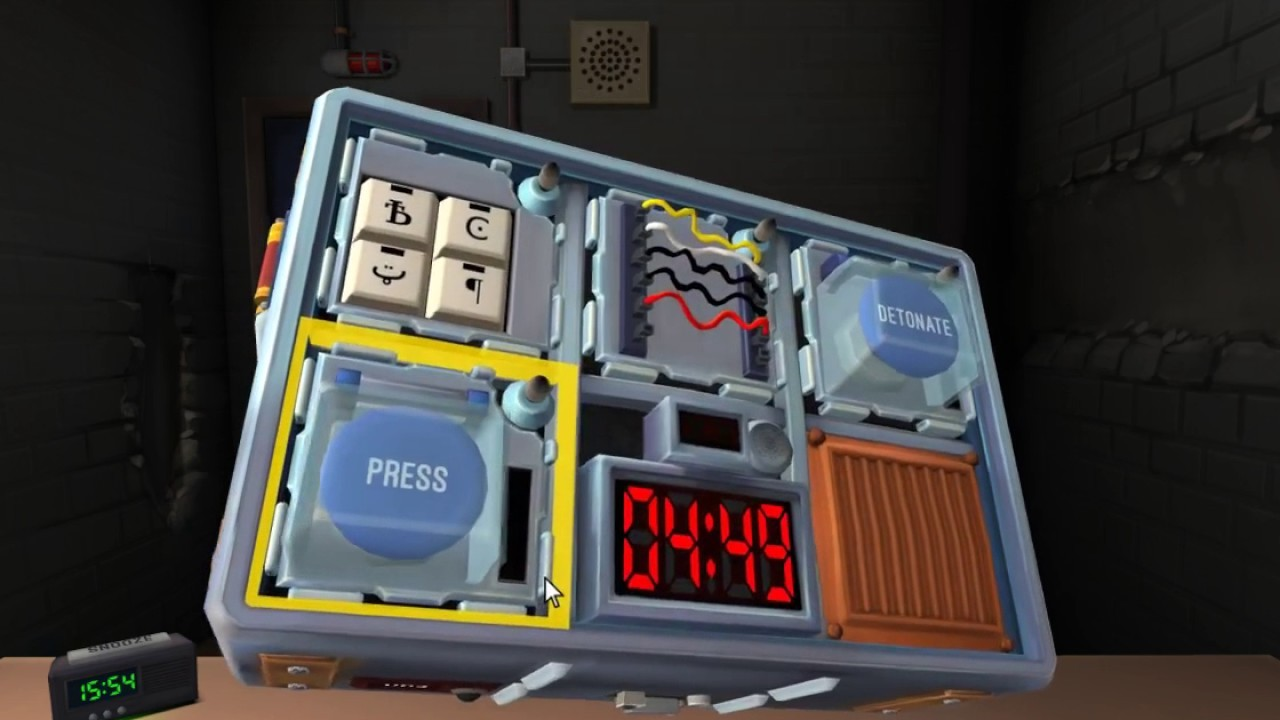
\includegraphics[width=\textwidth]{keep_talking_game}}

\vfill
\frame{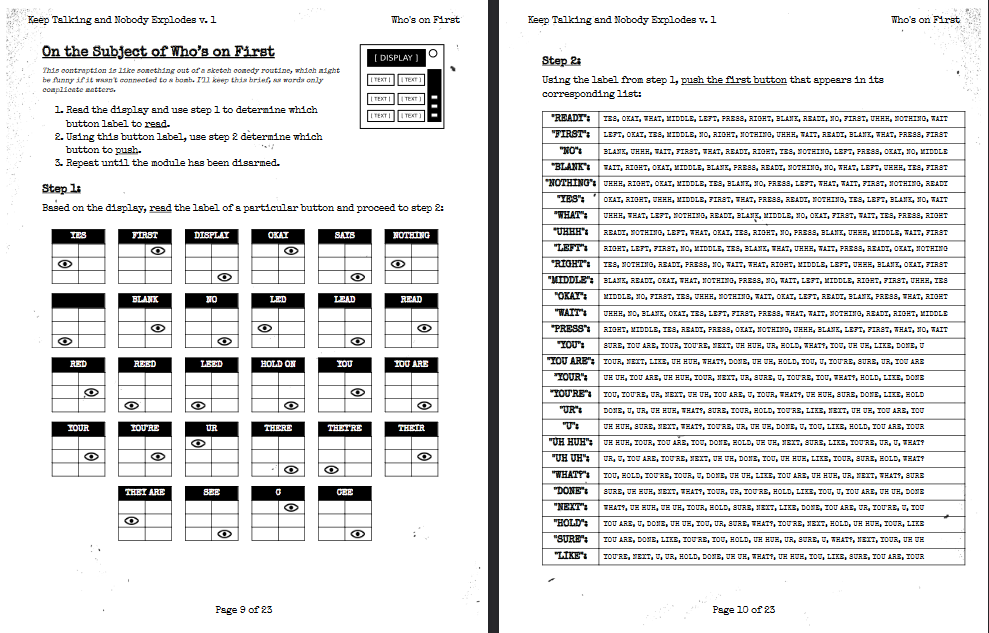
\includegraphics[width=\textwidth]{keep_talking_manual}}

\vspace{0.4cm}
The manual of the game is overcomplicated and explicitly designed to be convoluted. It contains the solutions to the puzzles, but they are obfuscated. Some players have simplified it and memorized it, so they can play without an assistant. This game is the most asymmetrical of the cited games. It's the main source of inspiration to the design of the game we developed. Both players need each other to complete the game, the manual player can't defuse the bomb and the defuser doesn't know how to solve the puzzles without having the manual memorized. This information unbalance is the basis of our game design.

\paragraph{Keep Talking and Nobody Explodes - Elevator of Doom \cite{ktneelevator}}
This is an example of how this game trained the players. A group of players of Keep Talking and Nobody Explodes completed a challenge called the "Elevator of Doom", which is a exceptionally difficult level. To finish in the 20 minutes time limit, the players spoke quickly in a condensed and clear manner to exchange the puzzles state and the solution. While the players learned how to beat the game, they also developed their communication skills.

\vfill
\frame{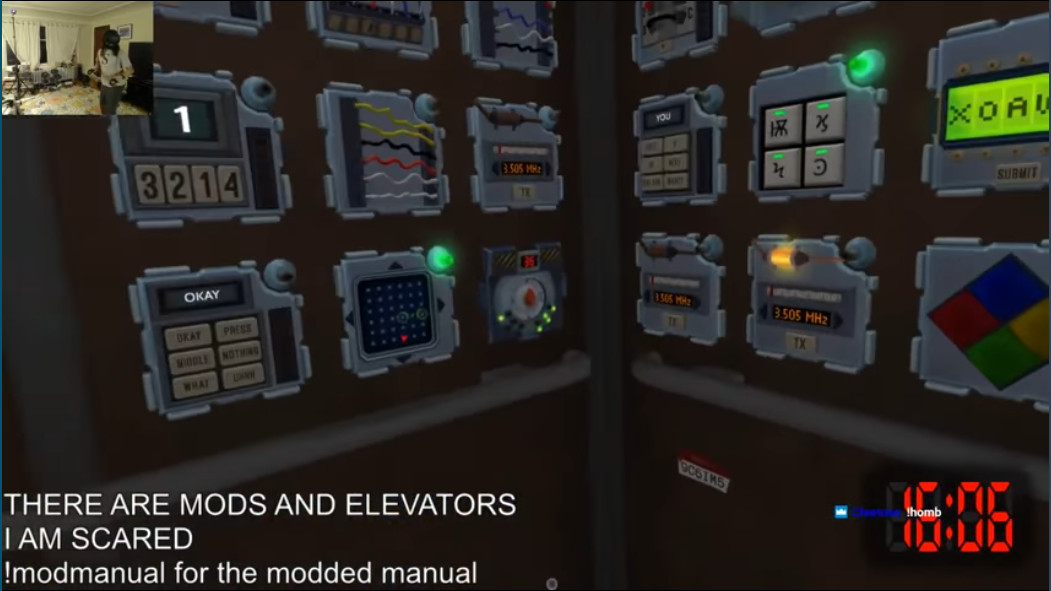
\includegraphics[width=\textwidth]{doom}}

\clearpage

\paragraph{Unrailed} \cite{unrailed}
The game consists in constructing a railway in front of a moving train. If the trains runs out of track, the game is over. In order to construct rails, the players have to chop trees, mine stone and combine materials in a specialized train cart. It's a 2 to 4 player game. The players  usually talk to split tasks among themselves and get time-sensitive tasks done quickly. This game is less of a serious game and is far more geared towards entertainment value: the puropose of the game isn't to learn external knowledge. However, players can use this game as a tool to improve their coordination, communication and reflexes.

\vspace{0.4cm}
\frame{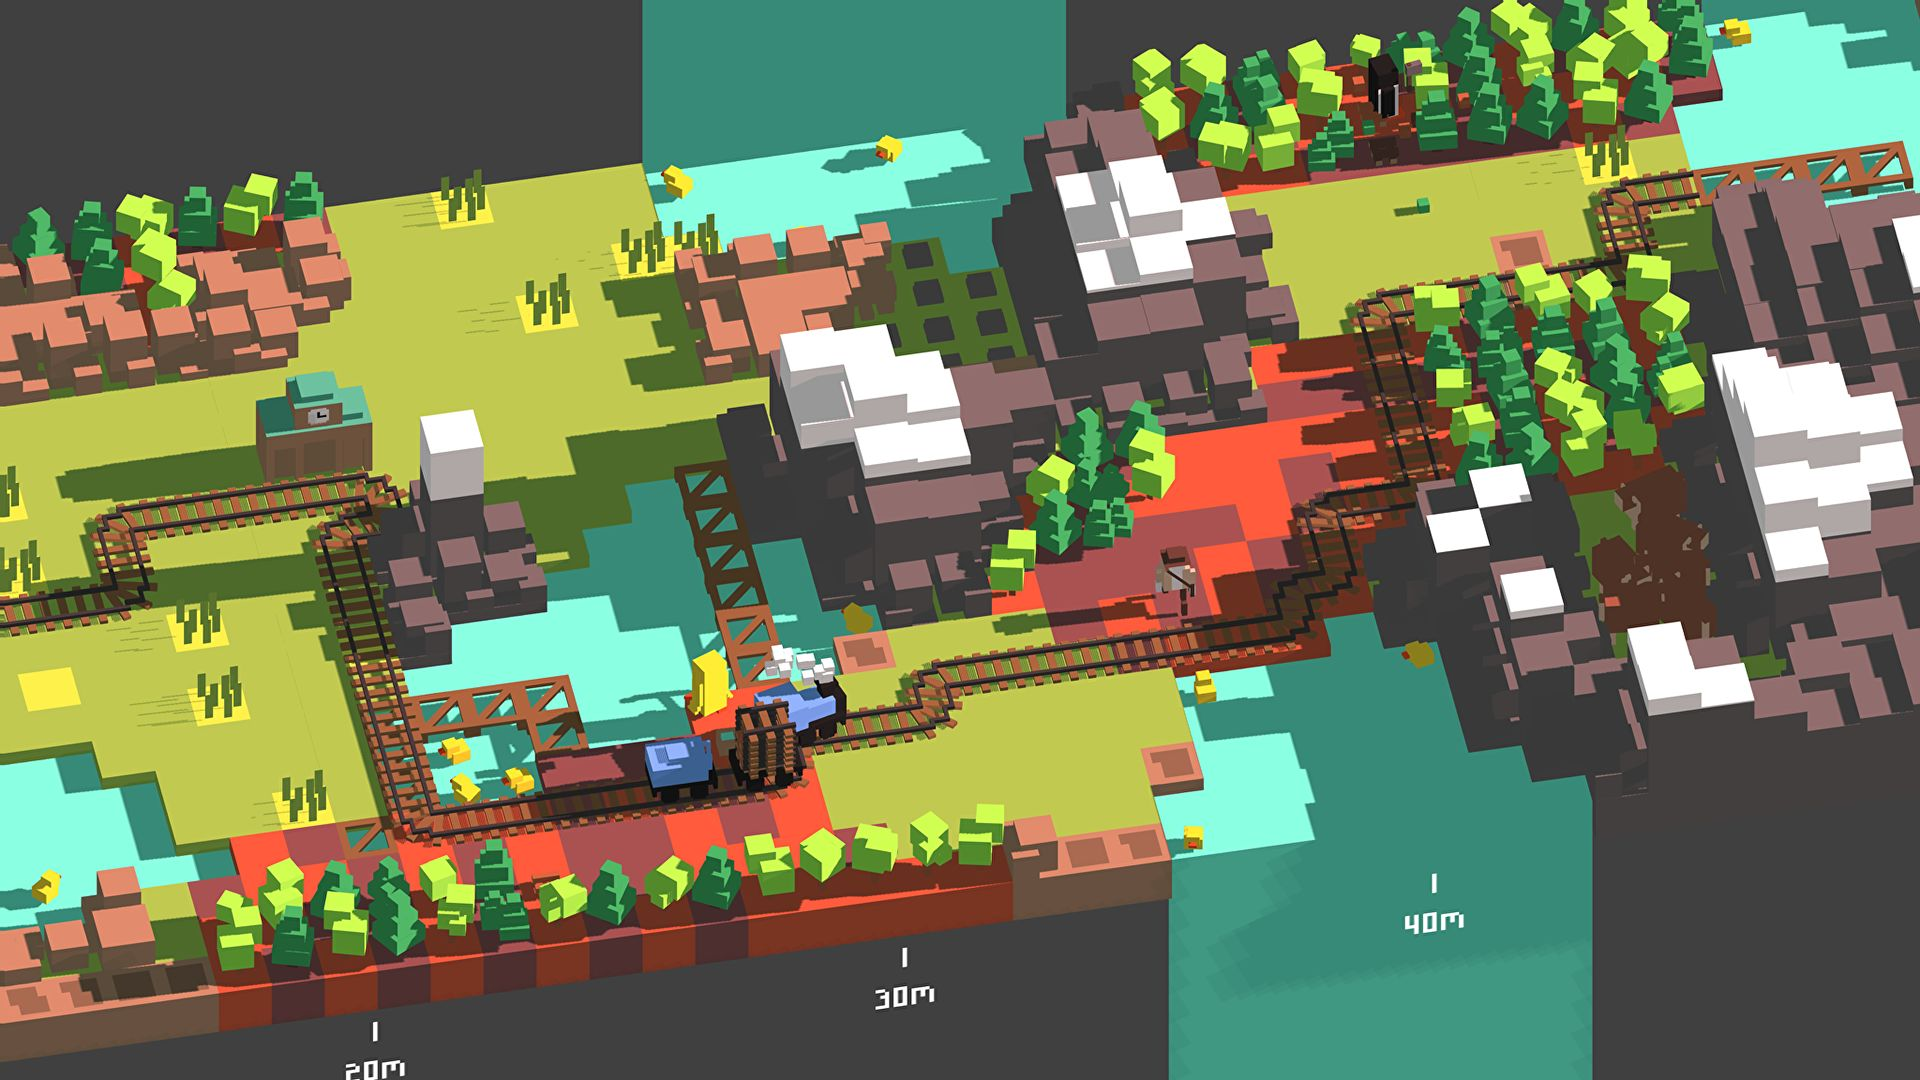
\includegraphics[width=\textwidth]{unrailed}}

\vspace{0.4cm}
The game includes pickups, scattered in the map and difficult to get. This pickups are used to upgrade the train and wagons. The upgrade screen is cooperative too, as the players can choose the upgrades by physically grabbing them.

\vfill
\frame{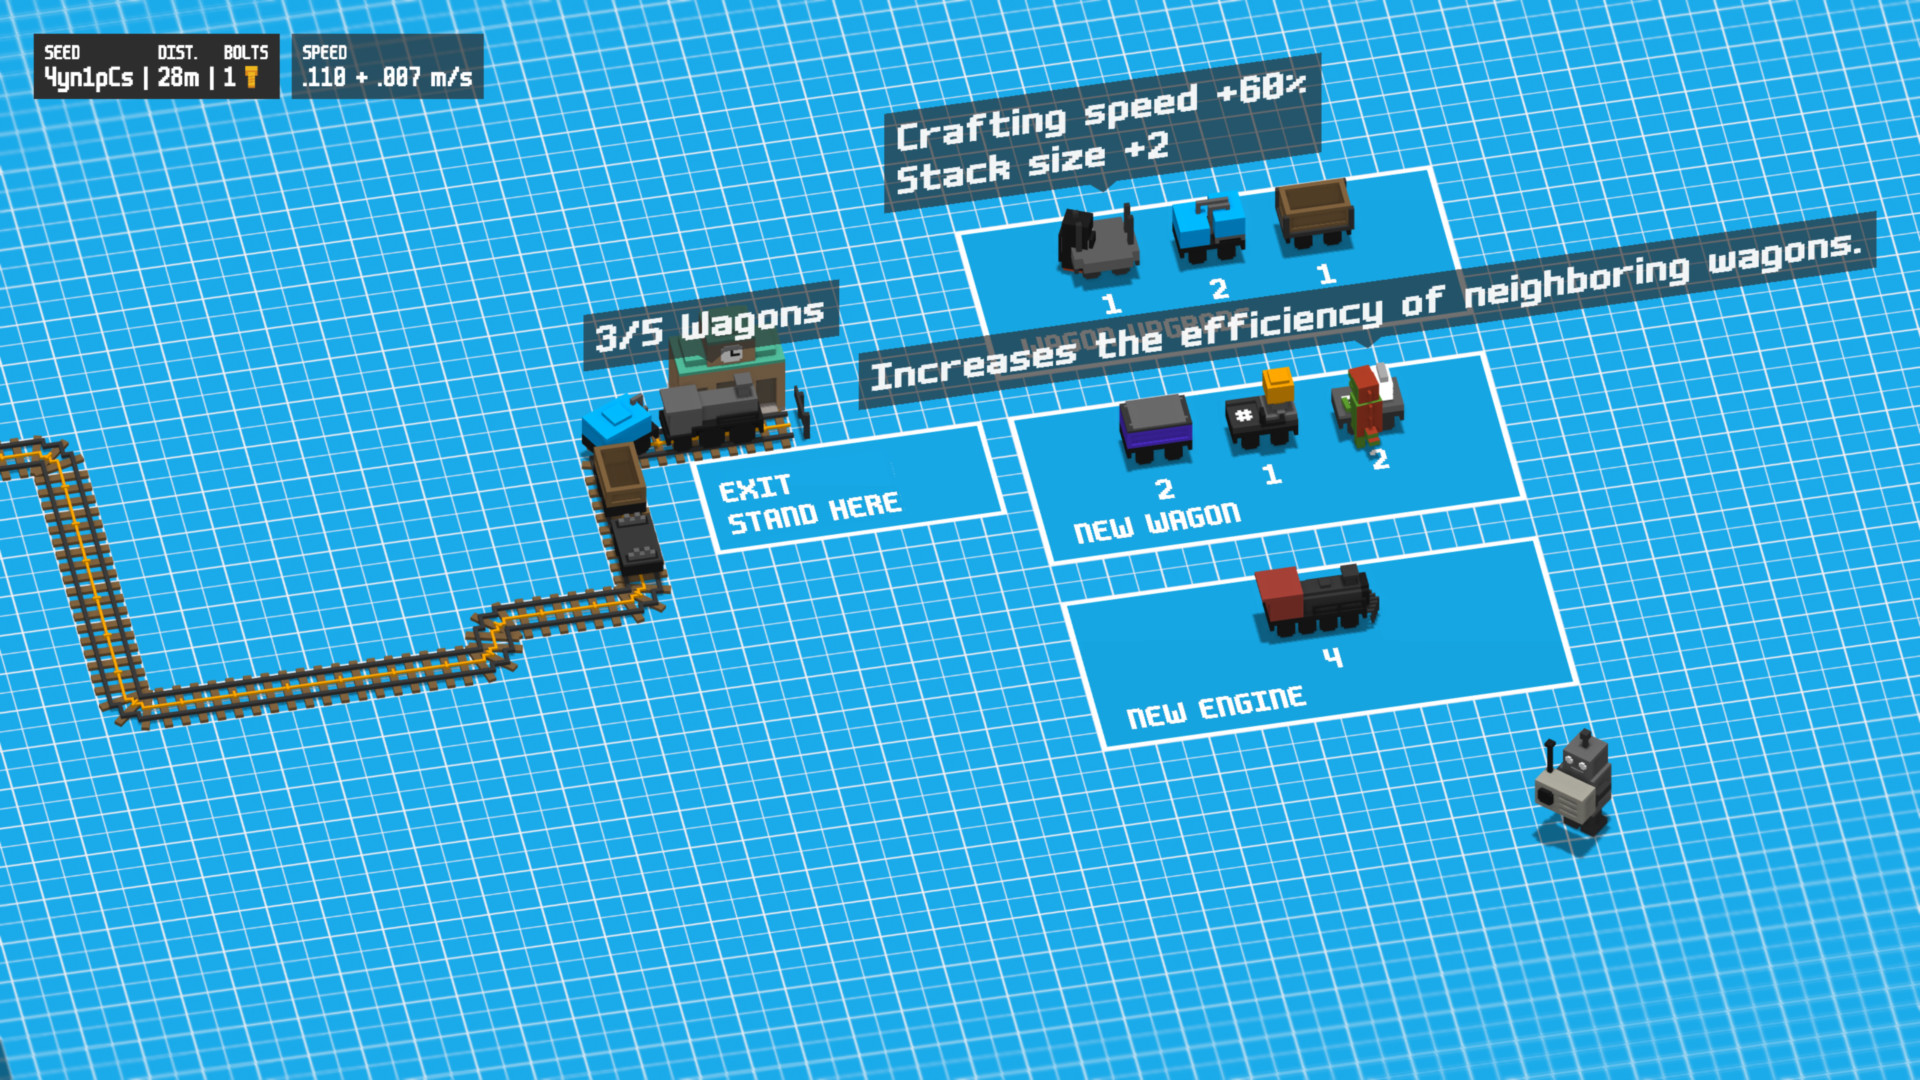
\includegraphics[width=\textwidth]{unrailed_upgrade}}

\clearpage

\paragraph{More Brain Training} \cite{mbt}
The game is a collection of puzzles that rate the player's mental skills. The game score is the mental age of the corrisponding average individual. The game is a serious game by design, it's purpose is to keep the player's mind sharp.

\vspace{0.4cm}
\frame{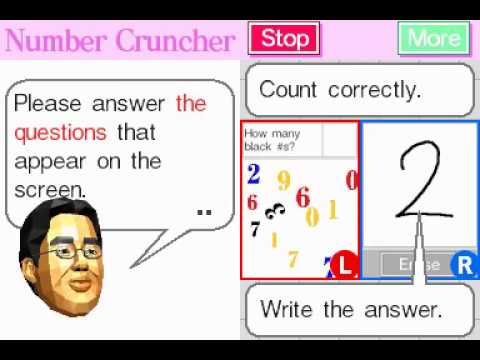
\includegraphics[width=\textwidth]{brain2}}
\vspace{0.4cm}

This game can be categorized as an exergame, term which is usually used for physical activity, for the mental training. However, the puzzles in the game are singleplayer and no speech is involved. The multiplayer aspect of the game is just the highscores, which can lead to competition which is not realtime.

\vfill
\frame{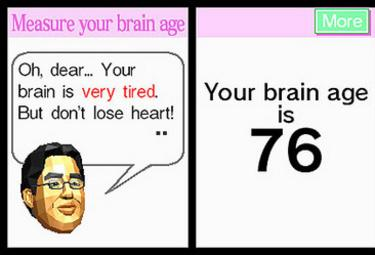
\includegraphics[width=\textwidth]{brain_age}}

\clearpage

\section{Game design}
The game is set in a city, with manhattan grid roads.
\begin{figure}[H]
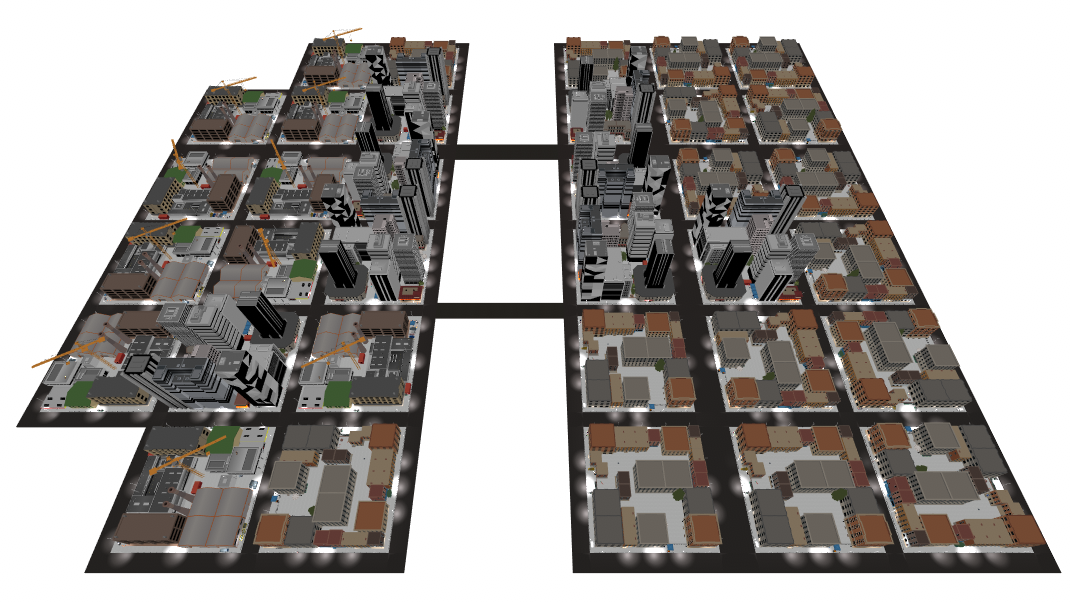
\includegraphics[width=\textwidth]{map_town}
\caption{One of the game's maps: Town}
\end{figure}
There are up to 2 couriers, which have to fulfil a list of delivery orders.
There is a master player who has a map, which shows the courier's positions and the street's traffic status. The master has the order list, the couriers do not.
The orders consist of a pickup site, a dropoff site and an item to be delivered.
The streets are blocked by many obstacles:
\begin{itemize}
  \item variable level of traffic makes the street difficult to navigate
  \item a drawbridge over a river
  \item sidewalk decorations
\end{itemize}
The master has to plan the route in realtime and relay the path to each courier in the broadcast channel based on the level of traffic.
The couriers drive following the Master path, they only see the pickup points and if they have picked up an item, the corrisponding dropoff point.
The game is lost if the players did not complete all tasks within the time limit, they win if they can complete all tasks.

\subsection{Traffic simulation}
The cars are agents that move thorugh a graph representation of the streets. The cars roam through the city by turning randomly at intersections. The cars respect traffic lights and occasionally will crash so that traffic jams happen dynamically.

\subsection{Items}
The items to be delivered are named and have two attributes: lives and weight. When the player has an item and crashes into a wall, the item is damaged. If the item is too damaged, the task is failed and the item reverted to the start. The weight of an item slows the player down by applying an acceleration penalty and a max speed penalty. The weight is not displayed in the game but it's effect are apparent to the couriers.

\paragraph{Item table}

\begin{center}
\begin{tabular}{ |c|c|c| } 
 \hline
 Name & Lives & Weigth \\ 
\hline
water bottle & 10 & 0.9\\
atomic bomb & 4 & 0.3\\
money bag & 12 & 0.7\\
cat & 9 & 1\\
glass panel & 3 & 0.5\\
hamburger & 6 & 0.8\\
box of fireworks & 2 & 0.4\\
apple & 7 & 1\\
pizza & 10 & 0.6\\
chandelier & 3 & 0.4\\
bowling ball & 15 & 0.1\\
candy & 8 & 1\\
pretzel & 10 & 1\\
bycicle & 12 & 0.4\\
saxophone & 6 & 0.8\\
 \hline
\end{tabular}
\end{center}

\subsection{Master's information}
The information that the master has of the players can be reduced in the settings. The master has three channels of information: geolocalization, video feed and audio from the radio. Turning off any of these channels the game becomes significantly harder, except when turning off the radio. The radio is essential for completing the game, so it cannot be switched off. Turning off the video feed and the geolocalization the master has no way of tracking where the players are, so the players have to constantly update the master with their position verbally. This exchange is made difficult by the half duplex radio, which jams if two players speak simultaneously.

\clearpage

\subsection{Interface design and menus}
The interface has been prototyped directly in Unity. The game is divided in the main menu and the game scenes. The interface is simple and intuitive, only the essential features to connect and play are present. 
\begin{figure}[H]
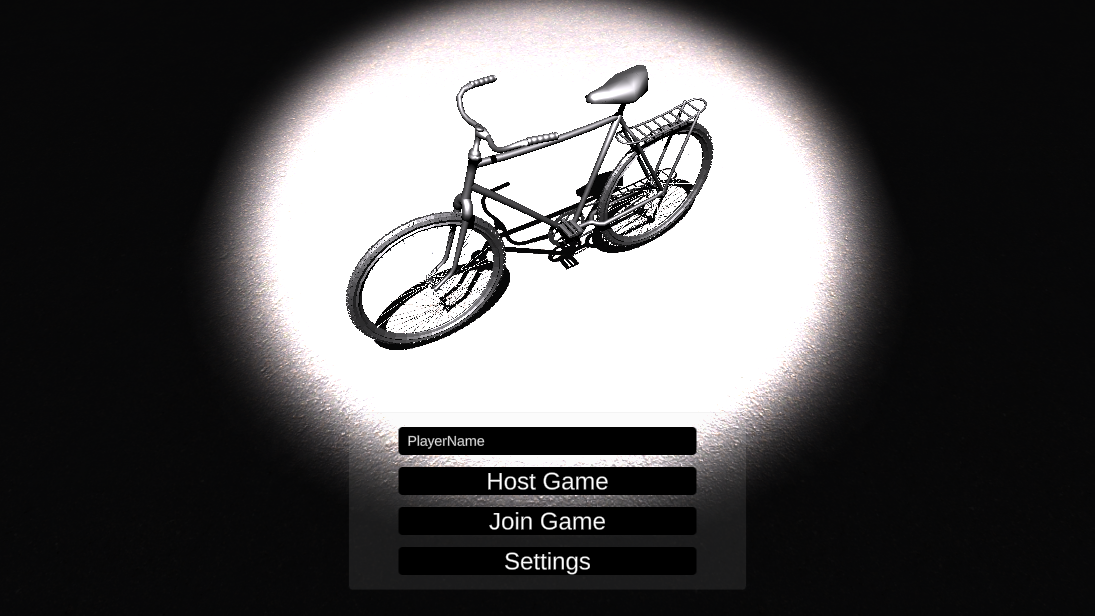
\includegraphics[width=\textwidth]{splash}
\caption{The main submenu}
\end{figure}
In the main submenu the player can choose a name and navigate to the lobby, settings and join submenu. \footnote{Bycicle model from Tidominer, \url{https://sketchfab.com/tidominer}}

\begin{figure}[H]
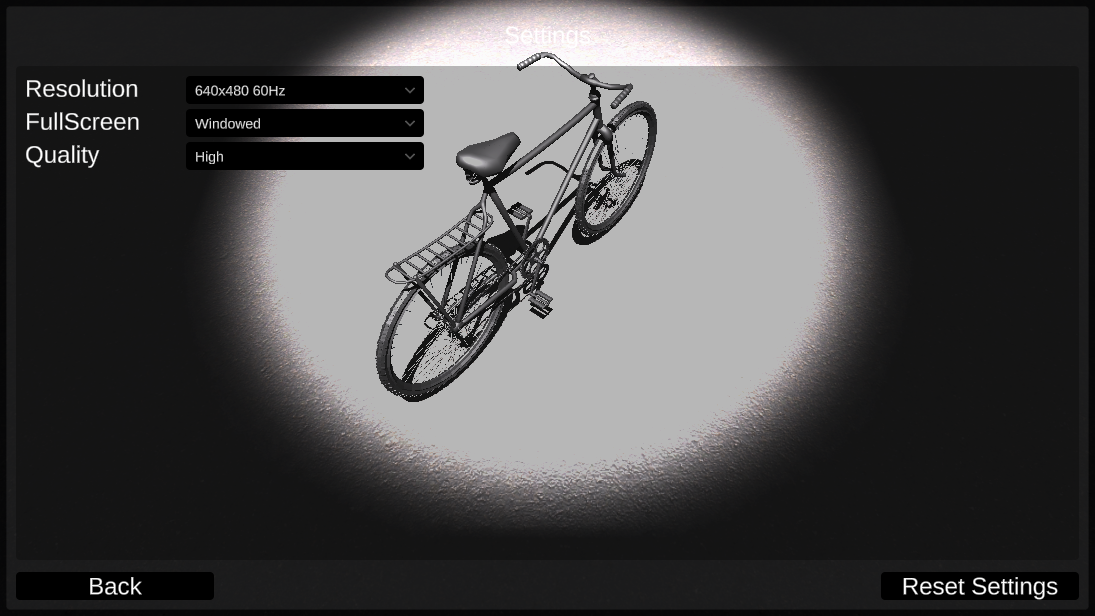
\includegraphics[width=\textwidth]{settings}
\caption{The settings submenu}
\end{figure}
The settings allows to control the game window, the game's graphic quality and the audio volumes. The menu is constructed dynamically and is easily expandable to accomodate for more options.
\begin{figure}[H]
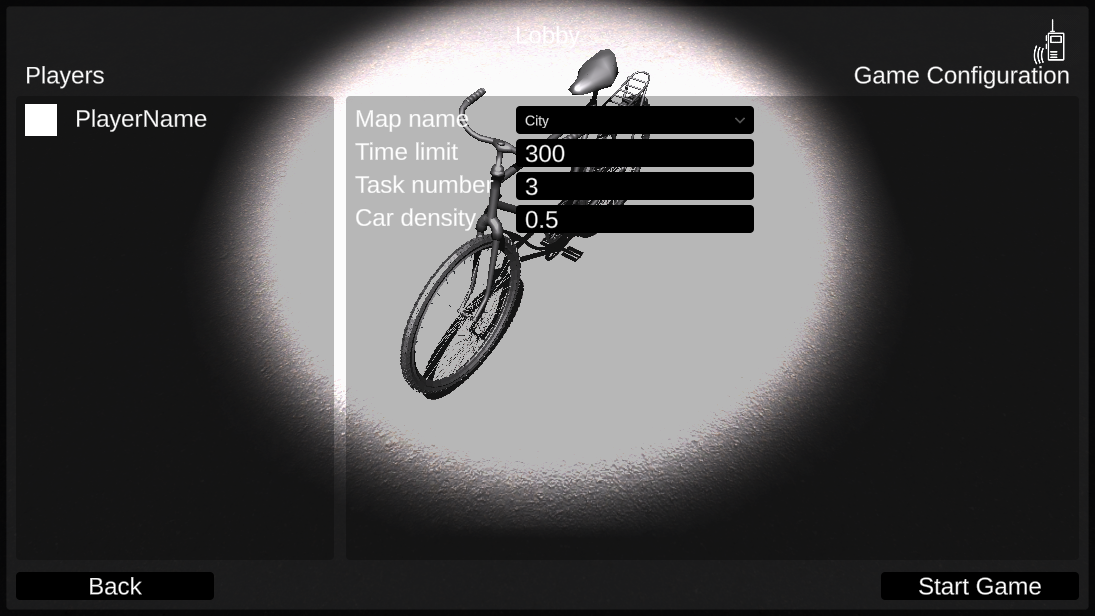
\includegraphics[width=\textwidth]{lobby}
\caption{The lobby submenu}
\end{figure}
The lobby is where the master (which is the host) accepts connections and configures the game. The players can see the configuration and chat vocally. The other players can't change the configuration but they can ask the master to change it. The configuration is constructed line by line with prefabs, allowing it to be quickly customized. Further development may be focused on automating the visualization of the configuration class by using reflections and getting a list of the arguments. The settings are constructed similarly.
\begin{figure}[H]
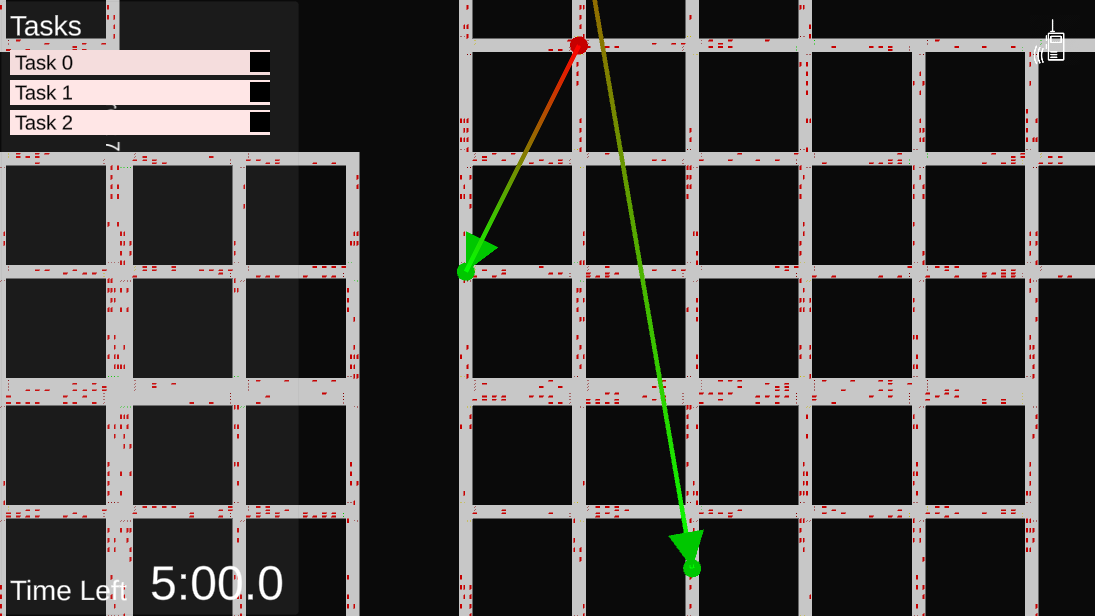
\includegraphics[width=\textwidth]{master}
\caption{The master interface}
\end{figure}
The master has at his left the task list and the time left in the game. In the bottom right there are the video feeds of the players and an arrow connects the feed to the corresponding player. The arrows which connects the pickup place and the dropoff of a task can be toggled by clicking on the corresponding task in the list. The task status (none, worked on, completed) changes the color of the task in the list.
\begin{figure}[H]
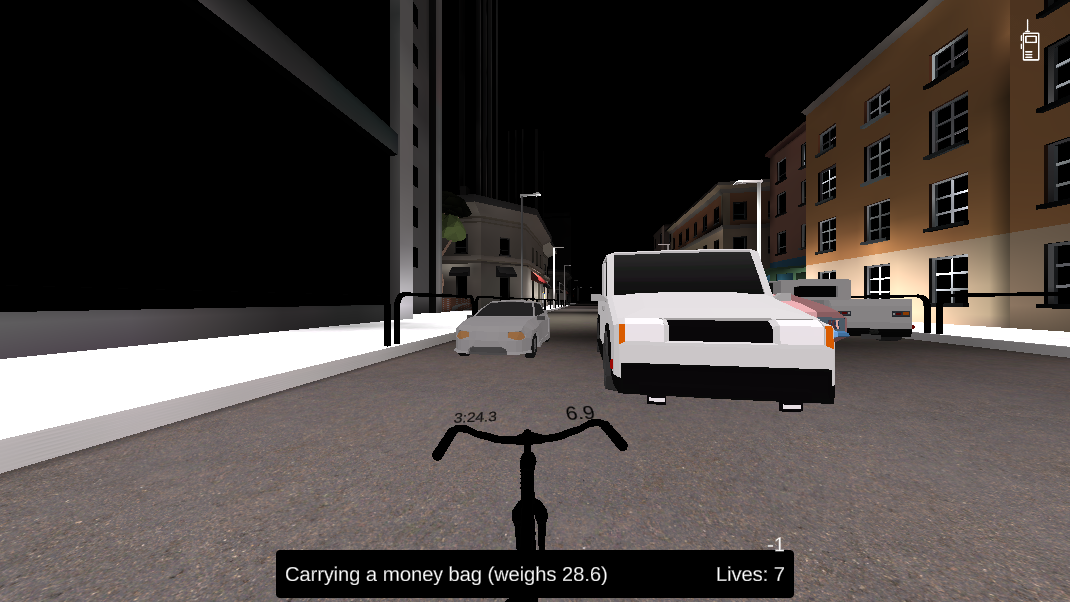
\includegraphics[width=\textwidth]{gameplay}
\caption{The player interface}
\end{figure}
The player can see the carried item name, the item weight and the amount of lives remaining until the item is broken. When a player loses a life an animation plays flashing a white vignette and decrementing the lives counter. The lower bar is the only visualization of the weight of the items. If the master wants to know it, he has to ask the player once the players has picked the item up. 

\paragraph{Radio visualizer}
In the top left of every screen (except the main submenu) there is the radio icon. This icon is animated based on the state of the radio connection, if the local player is transmitting and if the channel is jammed by too many people speaking.

\clearpage

\section{Implementation}

\subsection{Level design and 3D models}
\begin{figure}[H]
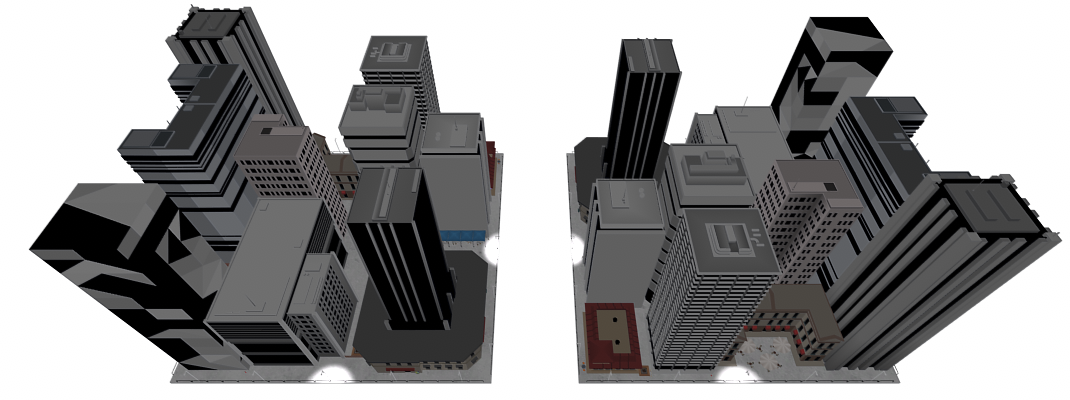
\includegraphics[width=\textwidth]{blockskyscraper}
\caption{Downtown block}
\end{figure}
\begin{figure}[H]
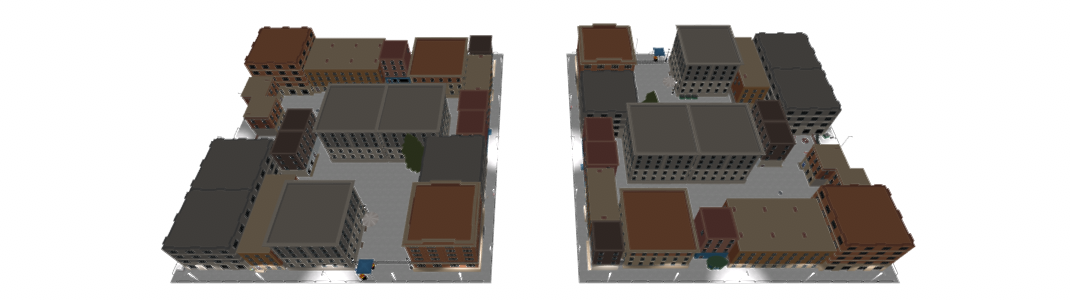
\includegraphics[width=\textwidth]{blockresidential}
\caption{Residential block}
\end{figure}
\begin{figure}[H]
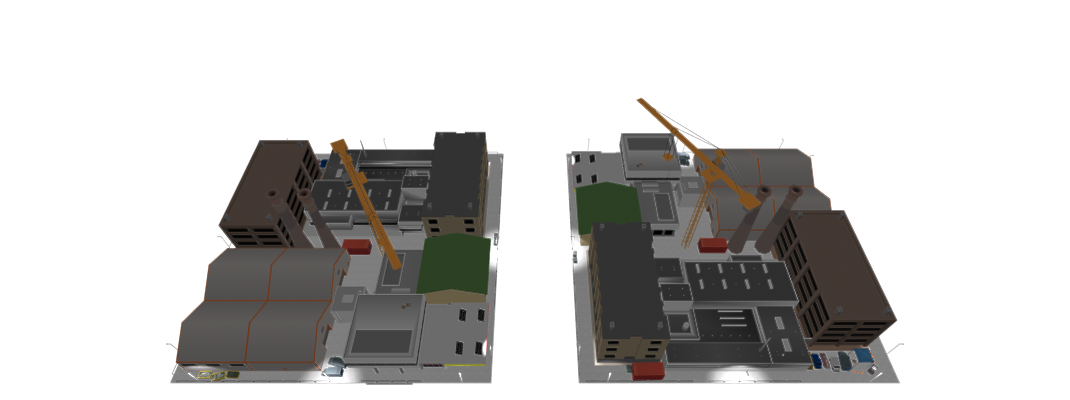
\includegraphics[width=\textwidth]{blockcargo}
\caption{Industrial block}
\end{figure}
The game maps are constructed by placing blocks, which are made of multiple buildings. Blocks are all contained in a square with a 110m edge. Blocks are assembled using the Everything Library \footnote{Assets from Everything Library © David OReilly, \url{https://www.davidoreilly.com/library}}. The roads are placed between blocks and their width is reflected in the number of lanes. Signs that indicate the names of the roads are generated following the road layout. Traffic lights and cars are generated at runtime. This workflow allows for big maps to be constructed quickly. In the game there are three maps: City, Town and Village. The maps are stored in separate scenes, so changes can be affecting only one map. This allows to have different lighting, decorative objects and gameplay elements.

\begin{figure}[H]
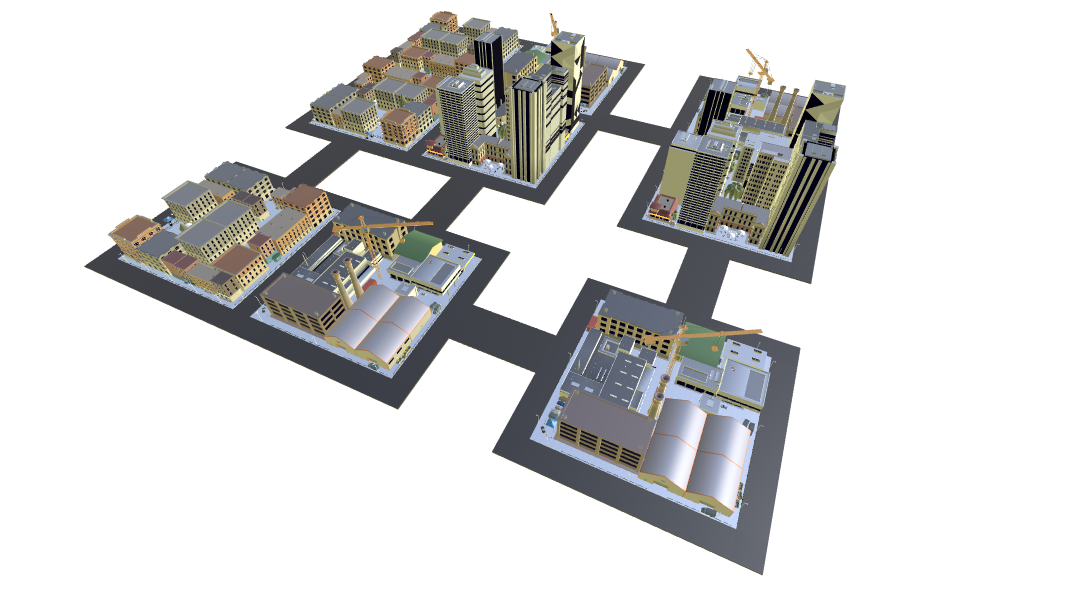
\includegraphics[width=\textwidth]{map_village}
\caption{Game map: Village. This map is the smallest and has the most bridges, the map is sunny and with a lot of ambient light.}
\end{figure}

\begin{figure}[H]
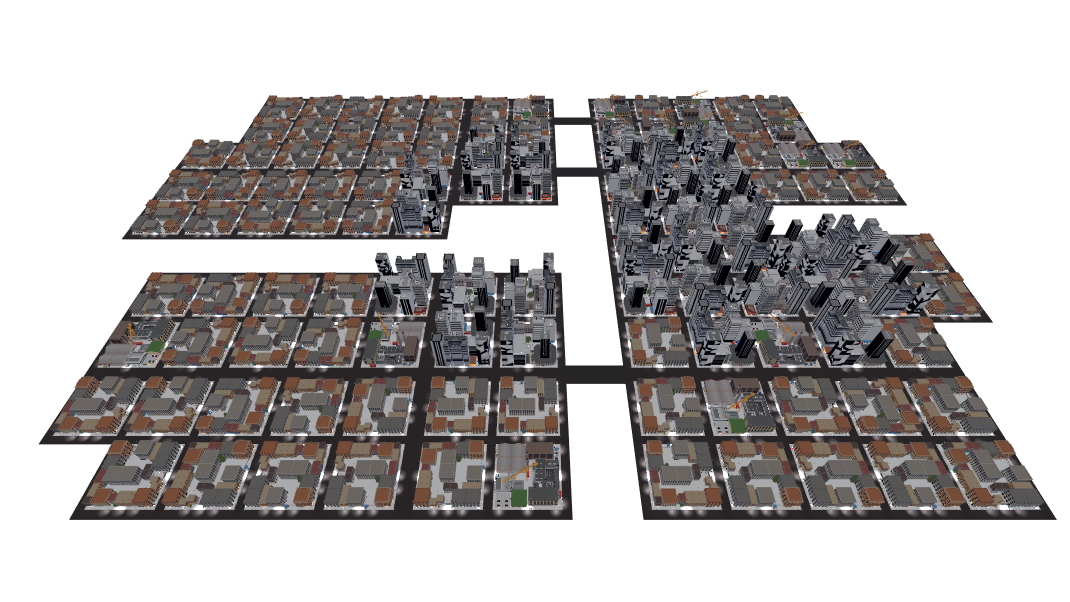
\includegraphics[width=\textwidth]{map_city}
\caption{Game map: City. This map is the largest and the most taxing performance-wise. The map is set at night with a lot of traffic lights and bright billboards lighting baked in.}
\end{figure}

\clearpage

\subsection{UDP Sockets with fragmentation, optional retransmission and integrity check}
The connection is handled using native C\# asynchronous UDP sockets. The network can send a message arbitrarily large (It will be fragmented into smaller packets). This system substitutes the deprecated Unity HLAPI (Unity Networking High Level API). Every message has a protocol number, which is used as a multiplexer allowing differently formatted messages to be sent along the same channel. The protocol is as follows:


\lstset{style=sharpc}
\begin{lstlisting}
public enum Protocol {
	normal, kill, ack,
	joinreq = 100, syncconf, start, 
	masterstate=1000, startgame, ready, 
	clientstate, over, 
	videoframe, 
	mastercars,
        radio=10000
}
\end{lstlisting}


If a kill is received, the network is shutted down. This functionality is used internally to exit from the networking callback cycle. Ack is used to send back a receive confirmation. The joinreq, syncconf and start protocol numbers are used by the lobby controller. The masterstate, startgame, ready, clientstate and over are used during the game. Mastercars is used to syncronize the initial state of the cars from the master to the clients. \\

\clearpage

\paragraph{Fragmentation}
If the message is longer than 1024 bytes, it's fragmented in parts no longer than 1024. Each part has the protocol, the serial number and the id along with an offset and a size. The offset is what part of the original is sent and the size is the size of the whole message. At the receiving end, the datagrams received are assembled back into the original messages using the serial number, the offset and size. The partial messages are stored in a dictionary indexed by the serial number and are made available externally only when full. If the fragments arrive not in order it isn't a problem as they are assempled based on their offset.

\begin{figure}[H]
\begin{center}
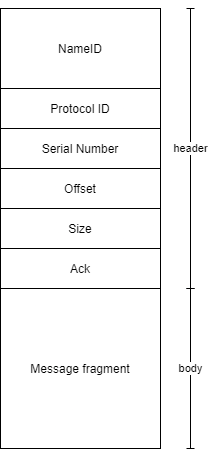
\includegraphics[height=8cm]{packet}
\end{center}
\caption{Network packet composition}
\end{figure}

\paragraph{Optional retransmission}
If the packet is marked as resend the system will wait for a response (ack) indicating that the packet was received. The system checks periodically if the timeouts of each packet is over. If the ack isn't received and the timeout is over the system will resend the packet with the same serial number.

\paragraph{Integrity check}
Each packet has a checksum byte to verify that the message has not been corrupted during transit. To generate the byte, the message is first assembled with the byte set to zero. The checksum is then set to 256 - the sum of all bytes. The receiver sums all bytes in the packets: if the sum is zero the message is correct. This technique is known as 1's complement sum \cite{checksum} and detects any single bit error, but has a lot of collision. A collision happens when the corruption happens to not modify the checksum.

\clearpage

\subsection{Game architecture}
The game is based on the model-view-controller pattern. \cite{mvc}
\begin{figure}[H]
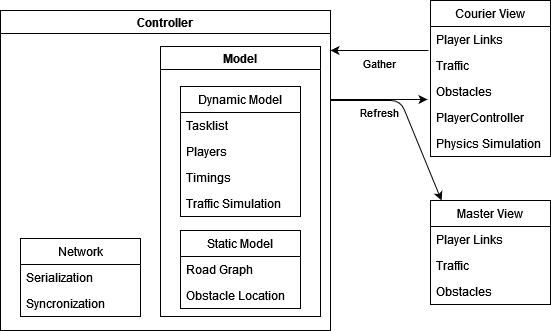
\includegraphics[width=\textwidth]{game architecture}
\caption{Game architecture diagram}
\label{fig:gamearch}
\end{figure}
\paragraph{Model}
A subset of the game rules which constitute the model are implemented decoupling the code from Unity. This subset is everything apart from the physics simulation, player movement and input management. The reason behind the separation from Unity is that the master mode has to be as light as possible. The master mode is meant to be able to run smoothly on slower devices and be ready to be ported to a native browser integration, which is much harder if it relies on some engine features. The model is divided into static and dynamic. The dynamic model is the state that changes during the game and is synchronized from the master to every client. The static model is loaded at the start and contains unchanging data.
\paragraph{View}
The view is split into master and client. In both instances, it creates a visual representation of the model and links each element to the model with it's identifier. When the model is changed, the view is updated.
\paragraph{Controller}
The controller interfaces with the model, the view, the networking and Unity. The controller behaves differently between client and master. The client gathers player data from and sends it to the master through the network. The master applies the client changes and sends back the updated dynamic model state. 

\clearpage

\subsection{Synchronization}
Multiple instances of a game can be synchronized either by passing only the inputs or the whole state.

\paragraph{Inputs synchronization}
By passing only the inputs, every instance has to update their simulation based on all inputs gathered before the previous update. As the master doesn't have a full simulation of the game (physics and player movement are only in the clients), this approach is unfeasible.

\paragraph{State synchronization}
The master sends the whole dynamic state to the clients. The clients pass the outcome of the inputs in the form of the player position and a flag if the player happens to collide with the enviroment. This approach is unfeasible if the state is too large to be efficiently sent tens of times a second over the network, but in this game's case the dynamic state is small enough.
\smallskip
\begin{figure}[H]
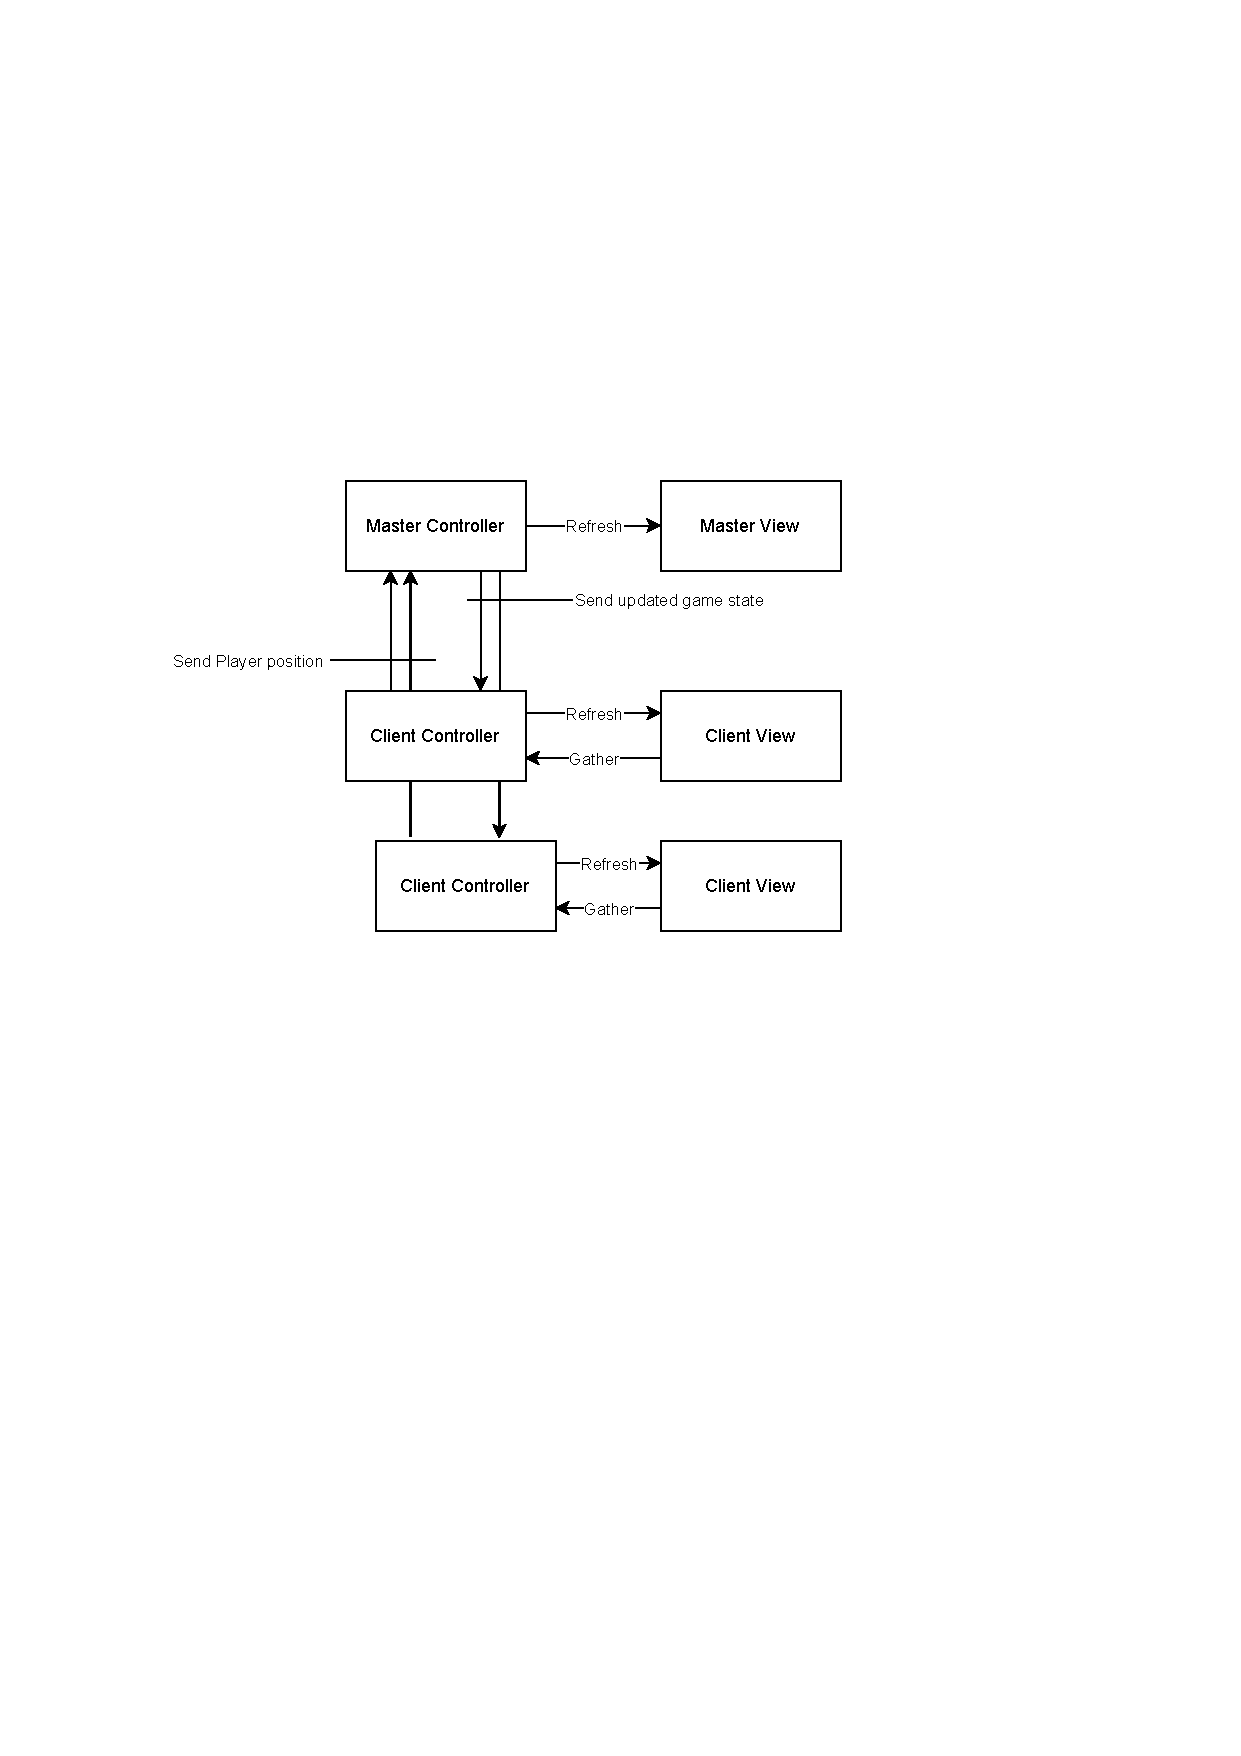
\includegraphics[width=\textwidth]{net architecture}
\caption{Network Architecture diagram}
\end{figure}
\smallskip

\subsubsection{Dead reckoning and latency hiding}
The network layer is unreliable and has variable latency. To mitigate for the delay and the unreliability there are multiple solutions: introduce a fixed delay or rollback.

\paragraph{Delay}
The fixed delay (usually less than 100 milliseconds) negates the variance in latency if the packets all arrive before the fixed delay. If one packet is late, every instance of the game must wait for the missing packet, ignore it and move forward without or rollback when it arrives.

\paragraph{Rollback}
When the server receives a late packet, it reverts the game state to the time it was sent and reupdates it back to the current time. While waiting for the late packet, the server computes the next states trying to predict the missing packet effects. This extrapolation, also called dead reckoning, can be effective with a trivial implementation when using input synchronization (use the inputs from the previous packet). The game uses state synchronization, so the extrapolation is nontrivial to define.

\paragraph{Extrapolation}
The extrapolation used in the game involves only the remote players position in the client view. The position is modified by the speed of the players based on how much time has passed since the last packet and the last speed known is kept constant.

\subsubsection{Advantages over HLAPI \cite{hlapi}}
Unity provides the multiplayer high level API which is a system that offers messages, serialization, state synchronization and network classes. HLAPI is deprecated and highly integrated in Unity, which is not desireable as it makes it very difficult to decouple the state of the game from Unity.

\clearpage

\subsection{Agent based traffic simulation}

\subsubsection{Definition and assumptions}
The agents of the simulation, cars, are defined by their position relative to a graph, a velocity and other paramters (random acceleration, random seed). This graph called "rail graph" is derived from the street level graph, which is a graph that defines the layout of the roads. The rail graph gets it's name from the cars behaving more like trains or trams, as they cant deviate from the rail graph edges. The rail graph is constructed by replacing every node of the road graph with an intersection and every edge with lanes. The road graph has a parameter for every edge indicating how many lanes the street has.
\begin{figure}[H]
\begin{center}
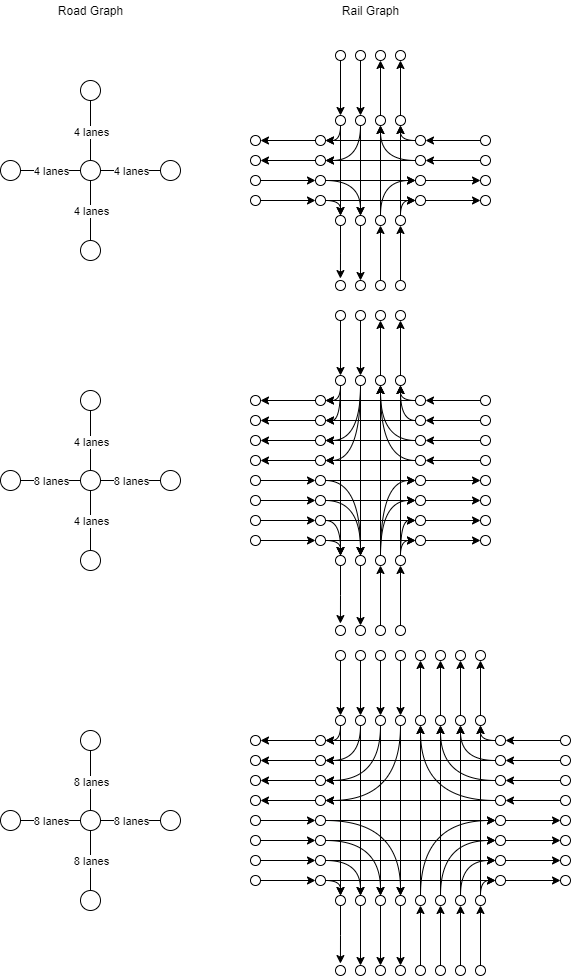
\includegraphics[height=18.5cm]{railgraph}
\caption{Rail Graph construction from the Road Graph}
\end{center}
\end{figure}
\bigskip 
 The rail graph is directed and the direction of an edge is the direction of the flow of traffic. At the intersection the rails are connected by bezier curves. The left turn rails are not connected to not allow cars to turn left, as it causes a jam instantly.
\begin{figure}[H]
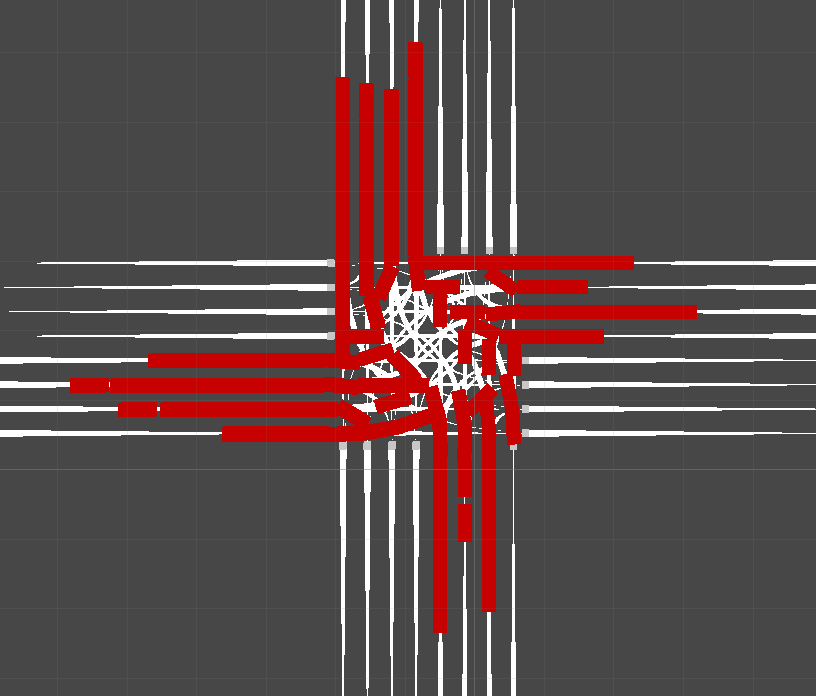
\includegraphics[width=\textwidth]{gridlock}
\caption{Left turn without traffic lights causes instant jam, this is the state after only 10 steps}
\end{figure}
\bigskip 
 To alleviate this jam, the left turning rails would have to be non intersecting and a left turn semaphore would have to be put in place. However, it is not necessary to do so as every point is still reachable without turning left.

\paragraph{Traffic lights}
Traffic lights are placed on the intersection's inward rails. This lights are coordinated at a street node level, so every traffic lights in an intersection is controlled by a single timer. Based on the position of this timer, the traffic lights states is set. The traffic lights are grouped into odd and even parity: odd parity lights are phase shifted by half a timer cycle. This grouping makes lights switch on and off based on their direction.
\begin{figure}[H]
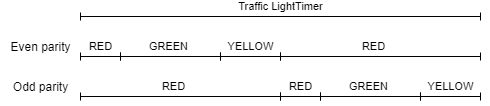
\includegraphics[width=\textwidth]{semaphore}
\caption{Traffic light timer and states}
\end{figure}

\subsubsection{Implementation}
\paragraph{Car-Train agent}
The car's position is defined by the starting node, the ending node (so the edge on which the car is) and the relative position \begin{math}{rel \in [0, 1]}\end{math} along the edge. The absolute position of a car is the position of the car within the frame of reference of the position of the nodes of the rail graph.\\
To get the absolute position a linear interpolation based on the relative position from the start to the end node is performed. If the edge on which the car is on is a bezier, the position is just the evaluation of the equation at the car's relative position.\\
To get the absolute direction the normalized difference of the end and start node is sufficient for the linear case. In the bezier case, the derivative of the bezier equation is the tangent vector, which normalized gives the absolute direction.
\begin{figure}[H]
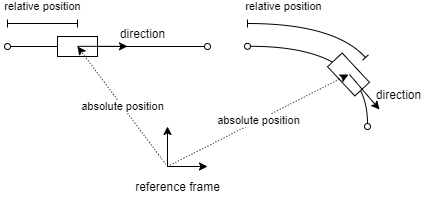
\includegraphics[width=\textwidth]{abspos}
\caption{From the relative position of a car to the absolute position and direction. Left: linear, Right: quadratic bezier}
\end{figure}

\paragraph{Integration}
The traffic state is a collection of cars. The state is integrated discretely with a time differential dt. Every car calculates how much distance it has to move by using it's velocity. This distance is then consumed by navigating the graph. The car's relative position is incremented by the relative distance, which is the distance divided by the edge length. This is easily calculated for linear edges, but bezier edges have a complex elliptical integral to solve to get their lenght \cite{bezier}. Therefore, the relative distance is calculated using an approximation of the bezier lenght by sampling a few points. \\
When a car reaches an intersection, if it has a red semaphore it stops. Otherwise, it chooses a rail based on it's initial random seed, which doesn't compromize the deterministic property of the simulation.

\subsubsection{Optimization}
\paragraph{Collision detection: lookahead dictionary}
Before the cars are moved, a lookup dictionary is constructed. This lookahead dictionary stores for every car the position it would have had if it moved some integration steps. The number of lookahead steps is a sensitive parameter with respect to number of incidents and runtime speed. Every time a car is moved, it checks if it would intersect any other future cars using the lookahead dictionary. If it would intersect, the car is stopped. \\
The intersection between two cars is an overlap check on two circles per car that approximate the bounds of a car.

\paragraph{Lookup optimization and caching}
Every collection used in the simulation can be accessed randomly in constant time and the absolute position and direction of a car are recalculated only when the relative position is modified. The rail graph has precalculated structures such as an index for accessing edges directly and a forward star collection for every node.

\paragraph{Intersection optimization: Grid indexing}
The intersection checking is the most costly operation for the simulation. In order to check faster, the cars further than a radius are excluded from the check. This is a coarse filter, but it requires a quadratic number of checks w.r.t. the number of cars. Therefore, an index based on the car's position is implemented. This index divides the space in a grid and for every square it has a collection listing all cars contained in the square. This index can be queried to return a neighbor of a car, and it does so by returning all cars in the original car square and all adjacent squares. 

\paragraph{Parallel integration}
The integration and collision detection algorithm can operate on a copy of the traffic state (which is a dictionary of cars) and apply the changes at the end of computation thanks to the lookahead dictionary. This makes it possible to parallelize the creation of the lookahead dictionary, the position integration and the collision detection. The threads have access to all the indexed data and traffic state and place their result into thread-safe containers. The threads work on a subset of cars and can't contaminate each other subset as they are changed at the end of computation.

\paragraph{Stopped cars linking}
The cars which are traveling and detect a still car on their path are stopped and linked to the other car. This link is broken when the car detects that the linked car is moving. When a car is linked to another, it's not needed in the lookahead dictionary and can skip being moved. \\
This linking procedure helps speeding up the intersection check, which is the slowest part of the whole simulation. Although, in the initial state the cars are placed in such a way that no car is linked, which forces the simulation to run slower until some cars are stopped in order for the linking procedure to take effect.

\subsubsection{Traffic synchronization}
The traffic simulation is synchronized by passing the current step of the master to the clients. The clients will advance their simulations until they reach the same step as the master, then wait until the master step is incremented. The initial state of the traffic model, which is composed of the cars and the traffic lights state, is sent from the master to the clients at the start of the game.

\clearpage

\subsection{Kinematic bycicle model \cite{kbm}}
The model is a simplified car steering model, where the front and back wheels are collapsed into one front wheel and one back wheel. The only steering wheel is the front one. \\
\smallskip
Known constants:
\begin{center}
\( l_r \) = distance from the center to the rear wheel \\
\( l_f \) = distance from the center to the front wheel \\
\end{center}
State variables:
\begin{center}
\( [x, y] \) = absolute position of the bycicle in the plane. \\
\( v \) = velocity of the bicicle. \\
\( \psi \) = heading angle \\
\end{center}
Control variables:
\begin{center}
\( u_1 \) = acceleration \\
\( u_2 \) = steering angle of the front wheel. \\
\end{center}
\begin{figure}[!h]
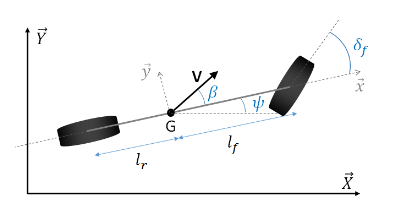
\includegraphics[width=\textwidth]{bike}
\caption{Kinematic bicycle model}
\end{figure}
\smallskip

\clearpage

The model's differential equations:
\begin{equation}\dot{x} = v \cos(\psi + \beta (u_2)) \end{equation}
\begin{equation}\dot{y} = v \sin(\psi + \beta (u_2)) \end{equation}
\begin{equation}\dot{v} = u_1 \end{equation}
\begin{equation}\dot{\psi} = \frac{v} {l_r} \sin(\beta(u_2)) \end{equation}
\medskip
where \( \beta(u_2) \) is the slip angle given by
\begin{equation} \beta(u_2) = \arctan (\tan(u_2) \frac{l_r} { l_f + l_r })  \end{equation}
\bigskip
The model is integrated discretely.
\begin{equation} x_{t+1} = x_t + \dot{x}\Delta t \end{equation}
\begin{equation} y_{t+1} = y_t + \dot{y}\Delta t \end{equation}
\begin{equation} {\psi}_{t+1} = {\psi}_t + \dot{\psi}\Delta t\end{equation}

\bigskip

\subsubsection{Player movement}
The player is moved following the KBM model. The Unity vertical and horiziontal input axis (which contain the standard movement input: arrows, wasd keys and gamepad sticks) are assigned to the control variables. 

\clearpage


\subsection{Radio}
The radio in the game is a simulation of a real half-duplex radio. This means that only one player at the time may speak. This is enforced by transmitting white noise while two ore more player are using the radio channel simultaneously. The simulation relies on a server based network to centralize the audio mixing process. All clients send their audio to the server, which mixes all the sources and sends customized mixes to each client and the local speaker. As a convention, all audio passing though the mixer has a sampling rate of 48kHz. 
\paragraph{Voice loopback}
The client audio doesn't loop back to the sender. When the voice returns to the speaker it's delayed, causing confusion. The server processes all audio sources to calculate if noise is needed, then for every client it mixes all sources except the client one.
\paragraph{Buffers}
The client audio is sent to the server and cached in a buffer in order to account for desynchronizations and network jitters. The server creates and fills a buffer for every client. Periodically, the server polls the buffers and mixes the polled data. The mix is sent to each client where it is cached in a buffer. This buffer is constantly polled by an Unity audio callback. The draining and filling of the buffers is balanced: the microphones produce as many samples as the ones consumed by the speakers, so the intermediate buffers serve as a transfer node. 

\begin{figure}[H]
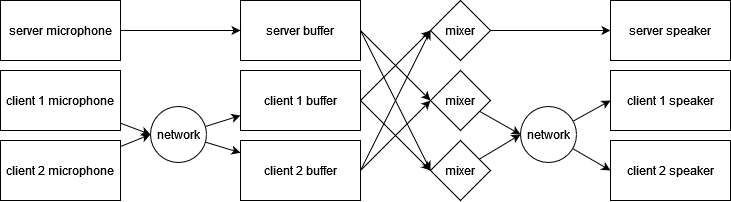
\includegraphics[width=\textwidth]{audio_mixer}
\caption{Audio pipeline diagram, the boxes represent the buffers.}
\end{figure}

\paragraph{Buffer delay}
Every buffers delays the signal by a set amount. This delay is crucial to alleviate the network variance, which otherwise would cut the signal and override samples. The buffers, when queried to read a certain amount of data, return silence if the data available is less than the requested amount. This ensures that the mixer will always have either a full set of data or silence and that the buffers will not cut the audio.

\clearpage

\paragraph{Sampling frequency and resampling}
The client's microphone may have a different sampling frequency from each other. The audio sent is resampled to 48 kHz and the audio received is resampled to the speakers sampling frequency. The sampler used is a custom sample and hold algorithm, it inserts or deletes samples following the ratio of sample rates.
\paragraph{Noise and Filters \cite{filters}}
The noise generated and mixed when multiple clients are speaking is white noise at 48 kHz. The audio generated by the clients is filtered by the server with a custom hi pass filter, which attenuates the low frequencies. This effect is done to make the simulation closer to an old style radio.\\
\begin{figure}[H]
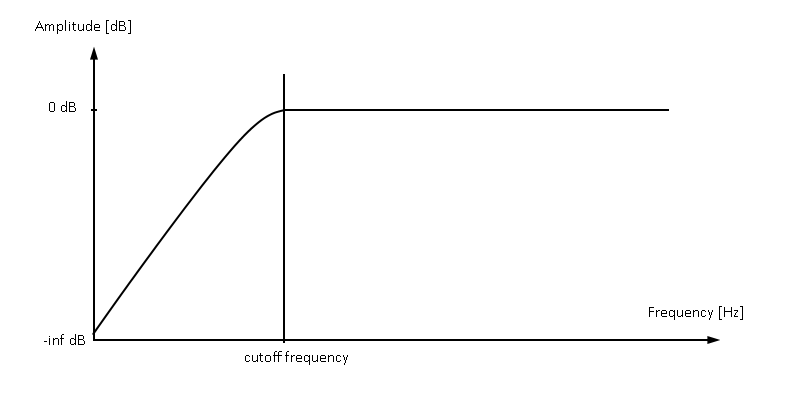
\includegraphics[width=\textwidth]{hipass}
\caption{Hi-Pass filter Bode diagram}
\end{figure}
\begin{figure}[H]
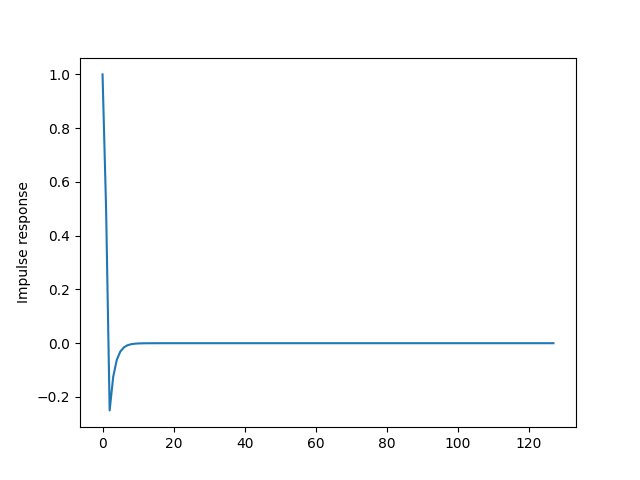
\includegraphics[width=\textwidth]{impulse_response}
\caption{Hi-Pass filter Impulse response}
\end{figure}
\bigskip
The filter is a recursive digital filter, defined by the following differential equation:
\begin{equation} y(n) =\alpha (y(n-1) + x(n) - x(n-1))\end{equation}

\subsection{Video}
The video feed is a frame of the player's camera which is sent to the master by each player. The amount of data required scales rapidly with the resolution of the frame and the frequency of the transmission.

\subsection{Editor tools}
The development process was sped up by the construction of tools for Unity. This tools are based on editor scripts, which allows to automatize some actions in the editors such as instantiating prefabs (keeping the prefab link) and destroying GameObjects.
\paragraph{Map generator}
The map generator places prefabs on a grid, randomizes their z rotation snapping on the 4 cardinal rotations and swaps these prefabs with their updated ones. This script also places road segments ensuring that no segment overlaps another and giving each segment a unique identifier.
\paragraph{Graph generator}
This tool generates a graph (a nodes and arcs tuple) from the elements present in the scene. The graph is saved directly in the Assets/Resources folder in json format. The graph can be visualized in the scene with a toggle in the script. The tool also visualizes the traffic rail graph, the cars and the traffic lights state. The traffic simulation can be stepped through directly in the unity editor, which eliminates the need to wait for unity to reset it's state while entering play mode. The tool can also place signs that display the name of the road at each intersection.

\clearpage

\section{Testing}
\subsection{Unit testing}
Unit tests are automated tests, they ensure that a small section of code behaves as intended. It's difficult to write testable code and to write tests for all the required functionality if the tests are not included in the design. To make it easier to write a complete test suite (set of tests of a program), a tecnique called test driven development is used to write code and tests.
\subsubsection {Test driven development \cite{tdd}} 
The model of the game is developed using the test driven development technique. This technique allows writing testable code by first writing a failing test and then the code to pass it. This makes the code more robust and easier to clean. Other aspect of the game such as the controller, the view or the map tools are not easily testable this way as they depend on the unity framework. One of the goals of TDD is to make it easy to refactor code: if the refactored code passes all tests the code is correct, there's no need to run it to know. This relies on the robustness of the test suite. If an essential functionality is not tested, the test suite is incomplete and by running all tests there is no guarantee of correctness.
\subsection{Integration testing}
The integration testing phase is largely done by hand. This is necessary as unity does't have a way to run multiple deployed instances inside a test environment. The testing routine is to deploy an executable and run it parallel to the editor instance. Some components are tested automatically, such as the serialization of the model and the interaction between smaller model components.
\subsection{Clumsy \cite{clumsy}}
Clumsy is a program that makes the internet network worse. It simulates packet loss, jitter, high latency, small bandwith, packet tampering. This tool is the basis on the game's retransmission and fragmentation algorithm, because it creates the perfect network conditions for testing. The packet tampering option highlighted the need to implement an integrity check for messages, which is necessary if the application is deployed on the web.

\subsection{System test and feedback}
The game as a whole was tested by indipendent testers. The testers rotated roles (courier and master), there was no more than one courier at a time and they were all set in the map "Village". The results are summed up in the following table:

\begin{center}
\begin{tabular}{ |c|c|c|c||c|c| }
\hline
	Time & Tasks & Video feed & GPS & Completed & Time left \\
\hline
	3 minutes & 5 & yes & yes & no & 0 \\
	3 minutes & 4 & yes & yes & no & 0 \\
	3 minutes & 3 & yes & yes & yes & 26 seconds \\
	5 minutes & 3 & yes & yes & yes & 131 seconds \\
	5 minutes & 3 & no & yes & yes & 95 seconds \\
	5 minutes & 3 & yes & no & yes & 10 seconds \\
	5 minutes & 3 & no & no & no & 0 \\
	8 minutes & 3 & no & no & no & 0 \\
	8 minutes & 3 & no & no & yes & 39 seconds \\
	8 minutes & 4 & no & no & yes & 154 seconds \\
	8 minutes & 5 & no & no & yes & 112 seconds \\
\hline
\end{tabular}
\end{center}

The testers started with a simple scenario and little time. They learned how to play (although they pointed out that the game doesn't explain itself properly) and were able to complete the game in under 3 minutes in just 3 tries. The game seems far more difficult when disabling both the video feed and the player's location (GPS). From that moment on, the testers had a much harder time speaking. The master had to rely on the courier telling him were he was otherwise he would have no indication of his position. The testers found the signs of the street names and were starting to learn the map, so they were able to beat the game consistently.

\clearpage

\section{Conclusion}
In this work we analyzed the usefulness of videogames as a learning tool. We designed and implemented a multiplayer videogame with an integrated radio that forces a rapid exchange of information between players to win. We developed a substitute for the default Unity Networking system (HLAPI) and a custom serializer that support large messages and is stable over adverse network condition. We developed a toolchain to easily produce maps from the Unity Editor. We used test driven development to implement the game rules. We designed and implemented a graph conversion algorithm and a parallel traffic simulation. \\

The system tests results show a significant improvement of the player's performance in the game. \\

For what concerns future development we will focus on the following:

\begin{itemize}
	\item Addition of environmental audio to make the traffic a more effecive obstacle.
	\item Addition of other obstacles such as railway level passages and pedestrians.
	\item Improvement of the traffic simulation by making it react to the players. 
	\item Port of the master code in javascript to deploy the master version in a browser. This step has been considered during design and the codebase has been written to make such a port possible.
\end{itemize}

\afterpage{\blankpage}

\clearpage

\bibliographystyle{plain}
\bibliography{references}

\end{document}
